\documentclass[pdftex,11pt,a4paper]{article}
\usepackage[english]{babel}
\usepackage{graphicx}
\usepackage[margin=2.2cm]{geometry}
\usepackage{fancyhdr}
%\usepackage[T1]{fontenc}
\usepackage{setspace}
\usepackage{multirow}
\usepackage{multicol}
\usepackage{mathtools}
\usepackage{amssymb}
\usepackage{caption}
\usepackage{url}
\usepackage{tikz}
\usetikzlibrary{arrows,decorations.markings,shapes}
\usepackage{array}
\usepackage{booktabs}
\usepackage{multirow}
\usepackage{pgfplots}
\usepackage{float}
\usepackage[font={footnotesize}]{caption}
\usepackage{graphicx}
\usepackage{todonotes}
\usepackage[font={footnotesize}]{subcaption}
\usepackage{listings}
%\usepackage[framed,numbered,autolinebreaks]{mcode}
\usepackage{graphicx,xcolor,textpos}
\usepackage{helvet}
\usepackage{placeins}
\usepackage{color} %red, green, blue, yellow, cyan, magenta, black, white
\definecolor{mygreen}{RGB}{28,172,0} % color values Red, Green, Blue
\definecolor{mylilas}{RGB}{170,55,241}
%\usepackage[]{mcode}


%\usepackage{hyperref}


\pagestyle{fancy}
\lhead{Reports ANN Jannes Nys (r0639870), MAI: Engineering and Computer Science}
\rhead{2015-2016}

\begin{document}

\begin{titlepage}
%\RequirePackage{fix-cm}

% ------------------------- Load packages ---------------------------
% You can eventually add these while you load other packages
% in case you want to integrate the titlepage with the rest of your thesis
% -------------------------------------------------------------------

% ------------------------ Page settings -----------------------------
% If you change these, the cover layout will also change.  In that
% case you have to adjust the latter manually.
% --------------------------------------------------------------------

\topmargin -10mm
\textwidth 160truemm
\textheight 240truemm
\oddsidemargin 0mm
\evensidemargin 0mm

% ---------------------- textpos settings ----------------------------
% Some additional settings for the cover
% --------------------------------------------------------------------

\definecolor{green}{RGB}{172,196,0}
\definecolor{bluetitle}{RGB}{29,141,176}
\definecolor{blueaff}{RGB}{0,0,128}
\definecolor{blueline}{RGB}{82,189,236}
\setlength{\TPHorizModule}{1mm}
\setlength{\TPVertModule}{1mm}

% ----------------------- Cover --------------------------------------
% Please fill in:
% - The title and subtitle (if applicable)
%         to include a formula in the title or subtitle
%         use  \form{$...$}
% - Your name
% - Your (co)supervisor, mentor (if applicable)
% - Your master
% - The academic year
% --------------------------------------------------------------------
\thispagestyle{empty}
\newcommand{\form}[1]{\scalebox{1.087}{\boldmath{#1}}}
%\sffamily
%
\begin{textblock}{191}(-24,-11)
\colorbox{blueline}{\hspace{139mm}\ \parbox[c][18truemm]{52mm}{\textcolor{white}{}}}
\end{textblock}
%
\begin{textblock}{70}(-18,-19)
\textblockcolour{}
\includegraphics*[height=19.8truemm]{LogoKULeuven}
\end{textblock}
%
\begin{textblock}{160}(-6,63)
\textblockcolour{}
\vspace{-\parskip}
\flushleft
\fontsize{30}{32}\selectfont \textcolor{bluetitle}{Artificial Neural Networks}\\[1.5mm]
\fontsize{20}{22}\selectfont Reports on Programming Assignments
\end{textblock}
%
\begin{textblock}{160}(8,153)
\textblockcolour{}
\vspace{-\parskip}
\flushright
\fontsize{14}{16}\selectfont \textbf{Jannes Nys} \\[4.5pt] Master of Artificial Intelligence: Engineering and Computer Science \\[4.5pt] r0639870
\end{textblock}

\begin{textblock}{160}(8,232)
\textblockcolour{}
\vspace{-\parskip}
\flushright
Academic year 2015-2016
\end{textblock}
%
\begin{textblock}{191}(-24,248)
{\color{blueline}\rule{550pt}{5.5pt}}
\end{textblock}
%
\vfill
\end{titlepage}

\tableofcontents
\newpage

\section{REPORT 1: backpropagation in feedforward multi-layer nets}
\subsection{Function approximation}
In this section, the goal is to approximate the function
\begin{equation}\label{eq:myfunction}
f(x) = \sin(x)\,,
\end{equation}
over the interval $[0,3\pi]$ using a linearly spaced vector as input, which covers the full interval with $50$ points. The standard number of neurons in the hidden layer is $5$. We train the network using a number of learning algorithms\footnote{In this report, we discuss batch learning algorithms. Online algorithms are not a part of the assignment. We only briefly mention that the online learning algorithms were found to converge faster, while the remaining MSE is larger compared to batch learning. This observation is in-line with the expectations.} provided by \texttt{Matlab}. Since the ability of a network to approximate a function depends largely on its architecture, we consider one function and network architecture for all learning algorithms.

\begin{figure}[htb]
\centering
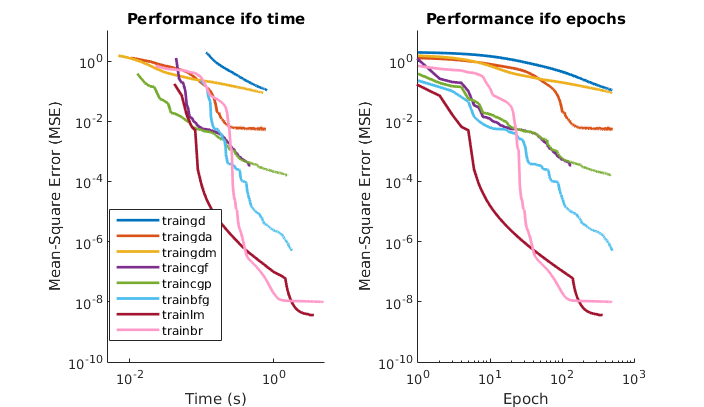
\includegraphics[width=0.65\textwidth]{figs/performance_plot.png}
\caption{Performance (MSE) of the tested training rules as a function of (left) time and (right) epochs where the maximum number of epochs is limited to $1000$. The log-log scale is opted to visualize the initial drop in MSE. \label{fig:performace_plot}}
\end{figure}

Below we compare the speed of various learning schemes, compared to the most basic gradient descent algorithm. We use the abbreviations of the algorithms, as used in the assignment.

\textbf{[traingd]} The gradient descent algorithm does not result in a proper approximation for most of the tested functions. The speed of each iteration evaluation is fast, but convergence is slow, and mostly never reached within $1000$ epochs. It is clear from the broad shoulder in the performance graph in Fig.~\ref{fig:performace_plot}, that an adaptive learning rate could significantly reduce the required time for convergence.

\textbf{[traingda]} Fixed step-size gradient descent has the following features: if the learning rate  is set too high, the algorithm can oscillate and become unstable. If the learning rate is too small, the algorithm takes too long to converge. An adaptive algorithm is an attempt to provide the best of both worlds by keeping the step size as large as possible, while allowing for smaller step sizes for locally complex error surfaces. This change is based on the performance of the network in the preceding epoch. 
In the first few ($\sim 10$) epochs, the performance is very similar as for traingd, yet, due to the adaptive learning rate, the MSE is reduced significantly after $100$ epochs, compared to traingd. This is reflected in an improved function approximation. Hence, approximate convergence is reached after fewer epochs. The time of an iteration is approximately the same as for the non-adaptive gradient descent. 

\textbf{[traingdm]} This algorithm includes a momentum term in the step. Momentum softens the learning algorithms' dependence on the small local variations of the error surface. It allows to jump out of a local minimum, while other methods get stuck. Except for this feature, the performance appears very similar in Fig.~\ref{fig:performace_plot}.

\textbf{[trainbfg]} This quasi-Newton method beats traingda by orders of magnitude (even after $10$ epochs, a clear difference is observed). Quasi-Newton methods build up second-order derivative information, based upon gradient information during the iteration process, allowing for faster convergence, while limiting the computational overhead.

\textbf{[traincgf]} and \textbf{[traincgp]} The conjugate gradient algorithms are usually much faster than variable learning rate algorithms. The considered conjugate-gradient methods perform very similar on the considered example. They only differ in the factor that determines the amount of influence of the momentum term in determining the next search direction. Then the next search direction is determined so that it is conjugate to previous search directions. These methods converge after just a few epochs, and combine this with a fast iteration step.

\textbf{[trainlm]} The Levenberg - Marquardt algorithm can be viewed as an adaptive mixture of a Newton-like and steepest-descent algorithm. By varying the $\lambda$ parameter in the step size $\Delta x = - (H + \lambda I)^{-1} g$, one can change which algorithm is dominant. The $\lambda$ is decreased after each successful step, converging towards Newton's method which allows for fast and accurate convergence close to an error minimum. This is clearly visible in the the performance plot in Fig.~\ref{fig:performace_plot}. When for a given $\lambda$ the step would increase the error value, the $\lambda$ is increased such that the error is always reduced. For the MSE function that is used in the network discussed here, an efficient approximation for the Hessian $H$ can be computed from the Jacobian matrix, which can be calculated much more efficiently. Altogether, the algorithm's design leads to a significant overhead in the speed of each epoch (factor of $\sim 10$ compared to traingd). However, the computational cost is fully justified, since for a minimum number of epochs, function \eqref{eq:myfunction} is properly approximated.
From the above analysis, the Levenberg - Marquardt algorithm shows to be the most suitable training rule to approximate function \eqref{eq:myfunction}, given the neural network architecture and the MSE error function. It is also the default algorithm of the \texttt{feedforwardnet} object.

\subsection{Generalization: noisy data and overfitting}
To simulate noisy data, we add a normally distributed noise to the original dataset, with standard deviation $\sigma = 0.3$. We map the bias and variance of the various methods considered in the previous section. This is done by generating $100$ data sets, and training a network with a given learning rule with at most $1000$ epochs. 
\begin{figure}[hbt]
\centering
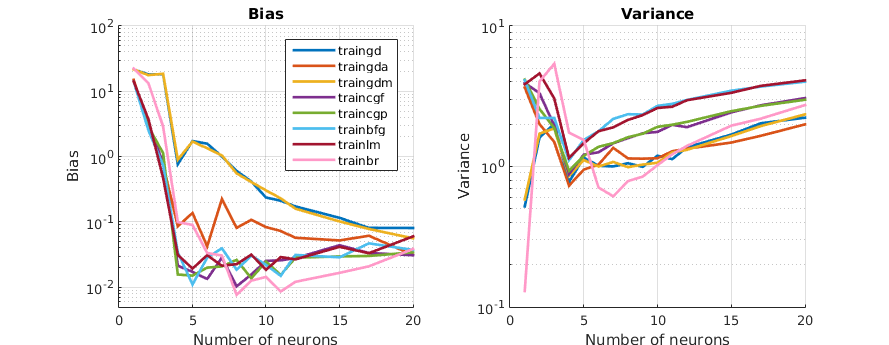
\includegraphics[width=0.9\textwidth]{figs/bias_and_variance.png}
\caption{Bias and variance as a function of the complexity of the neural network. In this exercise, \texttt{trainbr} can be ignored, since it is discussed in the next report.\label{fig:bias_and_variance}}
\end{figure}

Due to the fast learning property of the Levenberg - Marquardt algorithm, it now also requires more care to avoid overfitting. This is indicated by the large variance in Fig.~\ref{fig:bias_and_variance}. The more the network overfits the data, the larger the variation within the ensemble of networks, and the less generalizable it is. This can be avoided by e.g.\ early stopping, regularization or cross validation. More general, it appears that for different learning rules, with the same architecture and cost-function, the chance of overfitting is positively correlated with the speed of convergence (which was the topic of the previous section). 
Note that the bias of simple algorithms as traingd, traingdm and traingda result in a high bias. This is the result of the fact that these algorithms do not converge within 1000 epochs. This is also reflected in the low variance. 
Since `a strategy to avoid overfitting' is the topic of the next report, we refer the reader to that report for more details.


\FloatBarrier
\newpage
\section{REPORT 2: Bayesian learning in neural networks}
In this report, we discuss how Bayesian learning can be used as a method to avoid overfitting. Overfitting the noisy data in the data set of Exercise session 1 occurs when the resulted fit shows large gradients in order to reproduce every single data points (which minimizes the cost function). However, the principle of Occam's razor dictates that overcomplex systems should be avoided for simple problems. When complexity rises, errors on the validation set might increase, indicating overfitting. 

\subsection{`Pure' Bayesian training versus `trainbr'}
In the \texttt{perbayes} script, the weight values correspond to the MAP, i.e.\ the maximum of the posterior
\begin{equation}
\log P(\vec{w} | \mathcal{D}) = \log P(\mathcal{D} | \vec{w}) + \log P(\vec{w}) - \log P(\mathcal{D}) \,.
\end{equation}
for the data $\mathcal{D}$. Since the last term does not depend on the weight vector $\vec{w}$, we do not consider it in the following. Note that, if one compares this with the cost function $M$ in the assignment, we note that no hyper-parameters $\alpha$ and $\beta$ are included here. Therefore, we refer to this as the `pure' Bayesian algorithm. This is a restriction compared to the more general \texttt{trainbr} algorithm discussed below, where hyperparameters determine the effect of the prior and likelihood. These hyperparameters are also obtained from the data in a Bayesian way.

This first step of the exercise is mainly to see that regularization can be intuitively interpreted in a Bayesian framework. The reason for this is was illustrated above. However, without the inclusion of hyperparameters, we face a number of problems in the given simulation, which are to be avoided.

In order to better understand the need for the hyper parameters, we vary the number of data points in the data set. For a high number of data points, the influence of the prior on the posterior is negligible. However, the likelihood calculates the probability of generating a set of discrete values ($0$ and $1$), from a continuous distribution (a sigmoid in this case). Naturally, the optimization converges to a sigmoid function which is as sharp as possible, corresponding to a weight vector in the outskirts of its domain. In the limit of an infinite data set, the modulus of the weight vector is over estimated, and the direction is incorrect. The latter is due to the fact that the modulus of the weight vector is largest when $|\vec{w}| = \sqrt{2}$. Hence, a sharp boundary is favoured over a correctly aligned boundary. This is of course an effect of a limited range for the weight vector size. However, the main point is that the weights are over estimated. Overfitting of the network in principle corresponds to an overestimated $|\vec{w}|$. This effect we wish to counteract by introduction of the prior, which gives a higher prior probability of obtaining smaller values of $|\vec{w}|$.

For similar reasons, the MAP does not always result in a weight vector which is close to the weight vector of the original network. In most cases, the weight vector has an over estimated modulus. An example is shown in Fig~\ref{fig:example_perbayes}.  

For a low number of data points, the prior has too much effect, leading to a misclassification of a significant percentage of the samples.

Adjusting the effect of the prior properly can reduce this effect. Hence, introducing hyper parameters to scale the effect of the data and prior can improve the fitting. This is the case for the Bayesian regularization algorithm \texttt{trainbr}.

\begin{figure}[htb]
\centering
\begin{minipage}{0.2\textwidth}
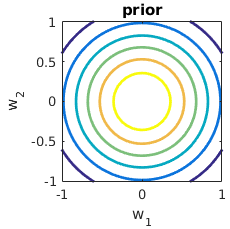
\includegraphics[height=3cm]{figs/prior_contour.png}
\end{minipage}%
\begin{minipage}{0.2\textwidth}
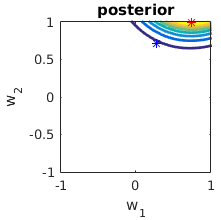
\includegraphics[height=3cm]{figs/posterior_contour.png}
\end{minipage}%
\begin{minipage}{0.2\textwidth}
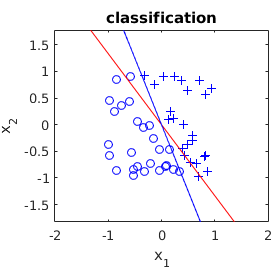
\includegraphics[height=3cm]{figs/separation_line.png}
\end{minipage}%
\caption{Prior, posterior and classification with corresponding separation line of the original (blue) and MAP network (red). Some (but not many) samples are misclassified.\label{fig:example_perbayes}}
\end{figure}

\subsection{Bayesian regularization using `trainbr'}
We now focus on the data set used in the previous report to discuss overfitting, and how Bayesian regularization may help reduce it.  An example of the effect of a Bayesian regularization term is illustrated in Fig.~\ref{fig:overfitting_example} where we compare the Maximum-a-posteriori result with a Maximum-Likelihood result.
\begin{figure}[htb]
\centering
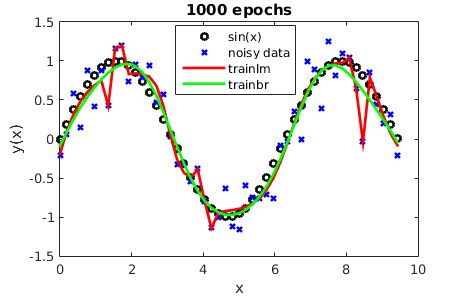
\includegraphics[width=0.5\textwidth]{figs/overfitting_example.png}
\caption{Illustration of an overfitted network trained with the Levenberg-Marquadt algorithm (red), compared to the results of the Bayesian learning (green) for a data set with $h(x)=\sin(x) + \mathcal{N}(\sigma)$ where $\sigma = 0.3$. Both networks have the same architecture, which includes $10$ neurons in the hidden layer.\label{fig:overfitting_example}}
\end{figure}
In the case at hand, in essence, we wish to approximate the underlying function $\sin(x)$ of the data, rather than the data set itself. In the Bayesian framework, regularization can be implemented in a natural way by opting for a parameter prior which has the bulk of its probability close to small values of the network weights (like a gaussian). 

In the last report we characterized generalization and overfitting via the network's variance and bias\footnote{Naturally, we could have also done this using a test set.}. We can therefore use the figure used in the previous report, now shown in Fig.~\ref{fig:bias_and_variance_plot}, and compare the \texttt{trainbr} algorithm with the other training algorithms. Figure~\ref{fig:bias_and_variance_plot} compares the bias and variance as a function of the complexity of the network for different learning algorithms.
 
\begin{figure}[hbt]
\centering
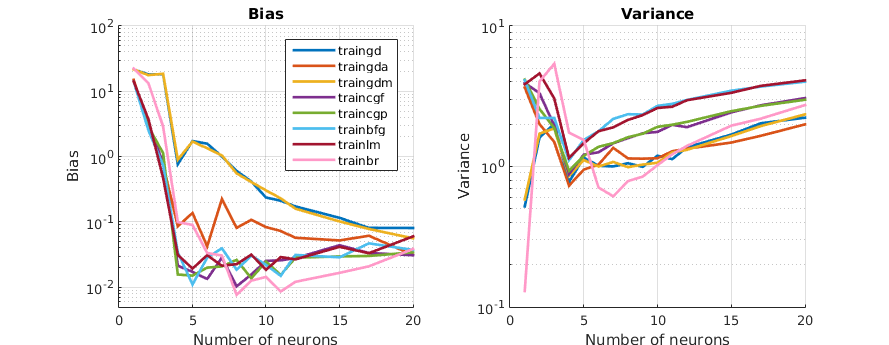
\includegraphics[width=0.8\textwidth]{figs/bias_and_variance.png}
\caption{Bias and variance plot as a function of the complexity of the neural network.\label{fig:bias_and_variance_plot}}
\end{figure}

An overfitted network corresponds to a low bias but high variance in Fig.~\ref{fig:bias_and_variance_plot}. Assuming convergence has been reached, a large variance indicates that the resulting network depends largely on the data set to which it is fitted, and hence, to the noise it includes. The effect of the Bayesian regularization term is most clear in the interval of medium complexity (5-15 hidden neurons). Both the bias and variance remain low, indicating that the \texttt{trainbr} algorithm allows for a more accurate and precise function reconstruction, while avoiding noise fitting (see again Fig.~\ref{fig:overfitting_example} for an illustration). Interestingly enough however, Fig.~\ref{fig:bias_and_variance_plot} also clearly shows the limited range of application of the Bayesian regularization. When the complexity is high enough, the regulation term has a negligible effect, and also \texttt{trainbr} will start overfitting.



\section{Report 3: Recurrent neural networks}
\subsection{Hopfield network for digit reconstruction}
In this section, we use a Hopfield network to reconstruct $15 \times 16$ pixel digits. Assume $p$ denotes the number of patterns stored and $N$ the dimensions of those pattern vectors. Since $p/N = 10/240$ is reasonably small, the probability of instabilities is small.

\begin{figure}[htb]
\centering
\begin{minipage}{0.08\textwidth}
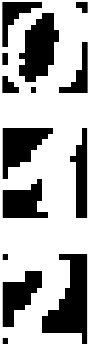
\includegraphics[width=0.9\textwidth]{figs/attractors.png}
\end{minipage}%
\begin{minipage}{0.08\textwidth}
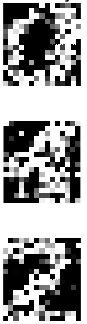
\includegraphics[width=0.9\textwidth]{figs/noisy_digits.png}
\end{minipage}%
\begin{minipage}{0.08\textwidth}
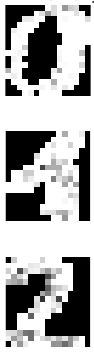
\includegraphics[width=0.9\textwidth]{figs/partially_reconstructed.png}
\end{minipage}%
\begin{minipage}{0.08\textwidth}
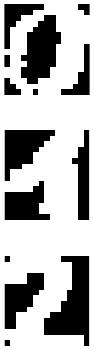
\includegraphics[width=0.9\textwidth]{figs/reconstructed.png}
\end{minipage}%
\caption{From left to right: attractor states, noisy digits, reconstructed digits after 1 iteration, reconstructed digits.}
\end{figure}

The retrieval states are the attractors of the system. They form the local minima of the associated energy function of the system. By distorting the original image (which is located at a local minimum), one increases the energy of the system (the image), allowing for a jump to a state (image) away from the original minimum. The higher the noise level, the less the distorted image resembles the original image. The Hopfield network is used to `cool the system down', lowering the energy along the geodesics defined by the weight matrix, such that it reaches a (local) minimum (or saddle points if one is unlucky). It can be shown that each step in a Hopfield iteration corresponds to a lowering of the energy of the matrix.
The final minimum can of course be different from the original one if distorting the image results in a state located in the attraction basin of another mode of the energy surface. In the following, we use the term `distortion energy' as the average energy that is added to the image during the distortion at a given distortion level.

When the noise level is low, the distorted image ends up within a small perimeter on the energy surface around the original image. Hence, in the majority of the cases, the image is properly restored.
When the distortion increases, the contour of the domain of distorted images increases in energy and hence in perimeter. The first false image reconstructions occur when the distortion energy reaches the same energy as the ridge separating its original minimum from another local minimum. In this case, when the distorted image is cooled down and energy is drained, it may end up in the wrong minimum. Hence, if this local-minima-separating ridge has a small energy (meaning that the two minima have a lot of resemblance), then this phenomenon will occur at low distortion.  For a noise fraction between $0$ and $1$, I observed no false reconstructions. However, if I increase the noise level above $1$, more interesting cases occur. The digits for which we first observe a false reconstruction when increasing the noise level, are at distortion level\footnote{The noise distortion level of the \texttt{hopdigit} function is supposed to be a noise fraction. However, nothing prevents us from taking values above 1.} $5$, for the `$2$' and `$9$'. These respectively end up in the `$7$' and `$2$' minimum in a large number of cases. This is expected, since these digits have similar features.

A second factor that needs to be taken into account is the number of iterations in the cooling process. If the number of iterations is too low, the system will not be able to fully cool down and will not reach a minimum. The maximum number of iterations should be large enough (such that the image results in an attractor state) and depends on the distortion level: the higher the distortion, the more steps are needed to guide the system to a local minimum. For the case at hand, $100$ iterations is generally sufficient.

A problem of Hopfield networks is that spurious states may occur. These are states which are not put in explicitly, but are generated from a linear combination of retrieval states. In the digit reconstruction, no such states were found in any simulation (even when the noise level is high). The reason for this is that it is unlikely to reach such a state, since it forms a perfect symmetry. We expect that clipping the initial noisy input would result in a higher probability to end up in spurious states. When the number of iterations is kept low, one can recognize combinations of digits in the reconstructed images. These states are close to the expected spurious states. 
%For discrete pixel values (e.g.\ black-white instead of the current gray scale), these spurious states would form a bigger problem. This is the case when the output transfer function \texttt{purelin} is changed to \texttt{sign} in the Hopfield network.

As a final test, we use other handwritten versions of the digits. These are also included in the \texttt{digits} workspace. Even with a low noise input, the Hopfield network can propagate to the wrong attractor state.

\subsection{Elman recurrent network approximation for the Hammerstein function}
First, the \texttt{elmants2} script was adapted. We generate time series set of 300 subsequent time steps. These are divided in two blocks with training:validation ratio 85:15. Note that, since we are working with a time series, the newelm uses blocks of subsequent time data instead of randomized indices. The test set is a sequence of 200 datapoints, separated from the initial set by 500 time steps.

In the documentation of \texttt{newelm}, \texttt{Matlab} makes the following interesting warning:
\textit{``Algorithms which take large step sizes, such as TRAINLM,
     and TRAINRP, etc., are not recommended for Elman networks.  Because
     of the delays in Elman networks the gradient of performance used
     by these algorithms is only approximated making learning difficult
     for large step algorithms."}

\begin{figure}[tbh]
\centering
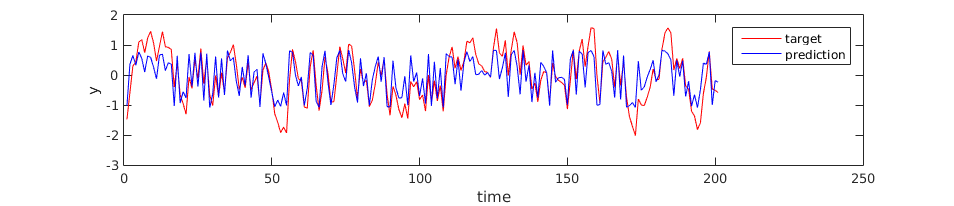
\includegraphics[width=0.8\textwidth]{figs/tansig_purelin.png}
\caption{Output of an Elman network with $10$ neurons in the hidden layer and the \texttt{tansig} and \texttt{purelin} transfer function in the hidden and output layer respectively. Also shown is the target test set. The correlation between both data sets is $0.795$. One should be aware that there is a time gap between the train and and test set. \label{fig:tansig_purelin}}
\end{figure}

In contrast to the non-dynamical case, where \texttt{trainlm} is often the default learning algorithm, \texttt{newelm} uses \texttt{traingdx} by default. This algorithm uses a gradient descent with momentum and adaptive learning rate backpropagation.

The use of the transfer functions as \texttt{logsig} is to be avoided, since its output domain is strictly positive. Especially when used in the output layer, the performance is low.

Even with the most simple architecture with \texttt{purelin} in the hidden and output layer, strong correlations ($>0.75$) between the prediction and target test set are obtained\footnote{In the following, we will refer to this correlation as `the correlation of the test set'. We opt to quantify the performance of a network on the test set by this correlation, since the underlying Hammerstein function models a stochastic process.}. Using the \texttt{tansig} transfer function in the hidden layer efficiently yields large correlations in the test set. However, it does not properly reproduce the outliers. This is illustrated in Fig.~\ref{fig:tansig_purelin}. However, we choose this configuration as the optimal one, since the test set correlation is maximal compared to all tested configurations.

In Fig.~\ref{fig:elman} we map the test-set correlation and MSE in function of the number of neurons in the hidden layer. From this plot, it is clear that the number of neurons must be limited to $< 20$ in order for the network to be generalizable.

\begin{figure}[htb]
\centering
\begin{minipage}{0.4\textwidth}
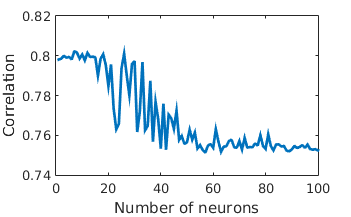
\includegraphics[height=3cm]{figs/correlation_map.png}
\end{minipage}%
\begin{minipage}{0.4\textwidth}
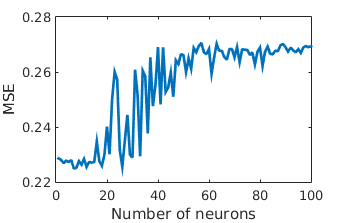
\includegraphics[height=3cm]{figs/mse_map.png}
\end{minipage}%
\caption{Correlation (left) and mean-square error (right) of the Elman network tested on the test set in function of the number of neurons in the hidden layer. \label{fig:elman}}
\end{figure}

\FloatBarrier

\newpage
\section{Report 4: Unsupervised learning: PCA and SOM}

\subsection{Principal Component Analysis on Handwritten Digits}
In the Principle Component Analysis, one decomposes the data entries into the principal eigenvectors of the covariance matrix. Each figure is then approximated by a linear combination (for linear PCA) of the limited set of eigenvectors. 

Two types of data were considered: non-standardized and standardized data. The former corresponds to the original data set, while in the latter, the data is preprocessed by putting the standard deviation of all pixels to 1. However, the data preprocessing was found to be less stable, resulting in higher reconstruction errors. Hence, we continue with the raw data below.

Figure~\ref{fig:recon_and_cumsum} shows the total reconstruction error for the data set of threes as a function of the number of eigenvectors used in a PCA projection. Figure~\ref{fig:recon_and_cumsum} also depicts the total sum of neglected eigenvalues. The figure illustrates that both quantities are proportional\footnote{Interestingly, the same simulation was also carried out without a standardized data set. In this case, the two curves in Fig.~\ref{fig:recon_and_cumsum} overlap exactly.}. Hence, by setting the required maximum reconstruction error, one can choose a proper number of eigenvectors of the covariance matrix to span the compressed space based on the cumulative sum of the eigenvalues.

When $k$ is equal to $256$, which is the dimension of the original basis, the eigenbasis of the PCA spans the full space of the original figures. Hence, the reconstruction error is approximately\footnote{Due to computational round-off errors, during the eigenvector decomposition and reconstruction, the obtained is not exactly $0$, but rather $6.7150 \times 10^{-29}$.} zero, since the PCA is now a rotation of the figures, which is inverted exactly upon reconstruction.

As an example, we show a reconstructed image for a number of dimensions of the PCA basis in Fig.~\ref{fig:reconstruction_example}. As the basis increases in dimensions, the reconstructed image converges towards the original image.

\begin{figure}[htb]
\centering
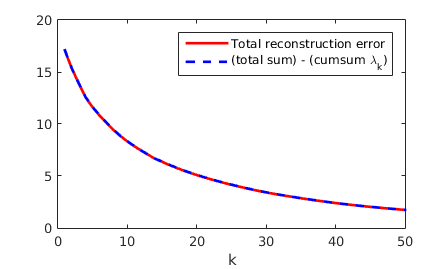
\includegraphics[width=0.5\textwidth]{figs/recon_and_cumsum.png}
\caption{Total sum of all eigenvalues minus the cumulative sum of the reconstruction $k$ largest eigenvalues of the covariance matrix (dashed blue) and mean-squared reconstruction error (solid red) as a function of the dimensionality of the PC basis.\label{fig:recon_and_cumsum}}
\end{figure}

%\begin{figure}[htb]
%\centering
%\subcaptionbox{Total sum of all eigenvalues minus the cumulative sum of the reconstruction $k$ largest eigenvalues of the covariance matrix\label{fig:cumsum}}{
%\centering
%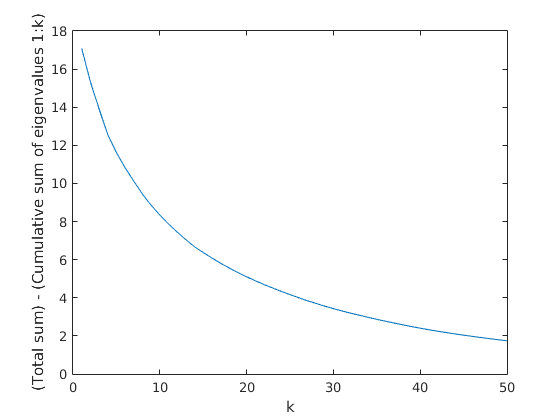
\includegraphics[width=0.48\columnwidth]{figs/cumsum.png}
%}
%\subcaptionbox{Total squared reconstruction error as a function of the dimensionality of the projection basis.\label{fig:total_recon_error}}{
%\centering
%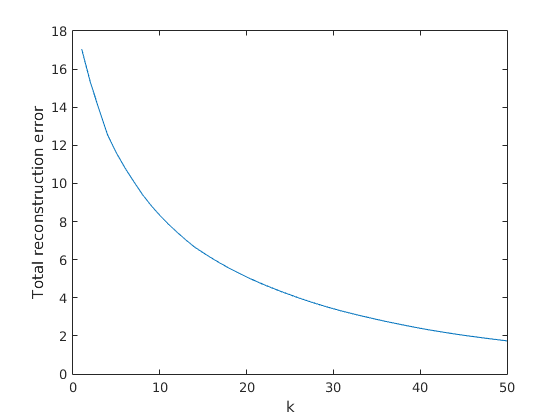
\includegraphics[width=0.48\columnwidth]{figs/total_recon_error.png}
%}
%\end{figure}

\begin{figure}[htb]
\centering
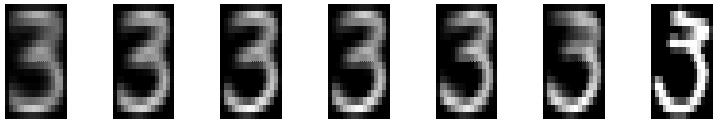
\includegraphics[width=\textwidth]{figs/reconstruction_steps.png}
\caption{Example of a reconstruction of an image using a basis of (f.l.t.r.) $1,2,3$ and $4$ principal eigenvectors. The outer-rightmost figure is the original, uncompressed image. It was observed that for this data item, a basis of $\sim 50$ eigenvectors is required to restore the image properly.\label{fig:reconstruction_example}}
\end{figure}

\subsection{Self-organizing maps: concentric cylinders}
Initially, a grid with a fixed (gridtop or hextop) or random (randtop) topology are generated. Using competitive learning, the weight vectors vary in such a way that they form a support for the concentric cylinder. The advantage of the fixed topologies is that these are easy to project onto 2D space, which makes the final result presentable. In this excersise, however, the purpose of the SOM is to represent the data density and topology using a lower number of vectors than the input data set.

It was found that fixed topologies generally have a number of weight vectors that remain in the center of the cylinder, while for `randtop' combined with `dist', this is not the case. The various distance measures in the representation space were found to have little effect on the general trends discussed above.

\subsection{Self-organizing maps: unsupervised clustering of the Iris data set}
The given example script \texttt{example\_SOM\_Iris.m} allows one to cluster the Iris data set given the prior knowledge that 3 different classes can be distinguished. More interesting is to run a SOM, without implementing such knowledge and using the SOM to retrieve structural information about the data set. This study is discussed below.
In this exercise, the benefits of a fixed topology are clear: it allows one to map a 4D data set onto a representable 2D figure. Hence, we opt for a 10 $\times$ 10 `hextop' grid and use the `dist' measure (the typical SOM rule of thumb suggests $5 \sqrt{N} = 61$ units for $N=150$). If too many weight vectors are included, many will never win and receive a hit. When the number of weight vectors is too low, the structure is washed out. The SOM adjusts its weights 1000 times. 

\begin{figure}[htb]
\centering
\begin{minipage}{0.40\textwidth}
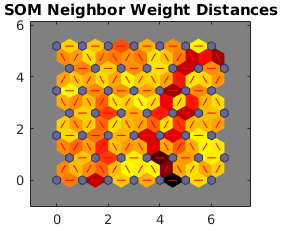
\includegraphics[height=4cm]{figs/som_distances.png}
\end{minipage}%
\begin{minipage}{0.40\textwidth}
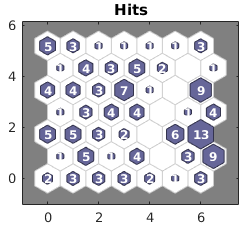
\includegraphics[height=4cm]{figs/som_hits.png}
\end{minipage}%
%\begin{minipage}{0.4\textwidth}
%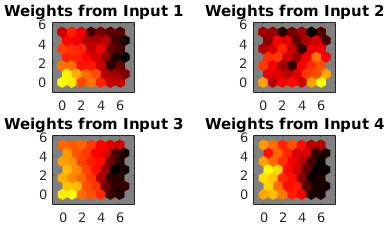
\includegraphics[height=4cm]{figs/som_correlations.png}
%\end{minipage}%
\caption{From left to right: neighbor weight distance (darker is further) and number of hits per weight vector.\label{fig:som_figs}}
\end{figure}

In Fig.~\ref{fig:som_figs}, we show the distances between the weight vectors, and the number of hits that corresponds to a certain weight vector. These visually indicate that there are two clearly distinguishable data types which are far apart in feature space 
%(this we know from the fact that we are using the `dist' measure). 
In between this region, there are a number of weight vectors that receive little to no hits. This also shows that, since we cannot clearly distinguish a third cluster, two cluster are located in each other's neighbourhood in feature space.

\FloatBarrier
\newpage

\section{PROJECT 1: Regression of function data}\label{sec:regression}
In this project, we use neural networks to approximate an unknown real scalar function $f:[0,1]\times[0,1] \rightarrow \mathbb{R}$, given a data set that was generated from this function. Since the underlying function is non-linear, a non-linear transfer function is required. Bearing in mind the results of Lehno \textit{et al.} \footnote{Leshno, M., Lin, V. Y., Pinkus, A., \& Schocken, S. (1993). Multilayer feedforward networks with a nonpolynomial activation function can approximate any function. Neural Networks, 6 (6), 861–867}, we find that the \texttt{tansig} (non-polynomial) function for the hidden layers must allow a function approximation if the number of neurons is sufficient. For the output layer, we use a \textit{purelin} transfer function, which does not restrict the output values to a particular range of values. In most cases, a single layer neural network is sufficient to reproduce a function (in theory, it is sufficient for \textit{all} functions if the number of neurons is large enough). Hence, we start with a single layer. Since the typical Euclidian distance between data points is small compared to the typical dimension of the spatial structure ,  in addition to the fact that the data has not been jittered, the number of neurons can be taken relatively high without overfitting. To get an estimate of the number of neurons, we refer to Fig.~\ref{fig:performance_val} where we map the MSE of the training and validation set as a function of the number of neurons in the hidden layer\footnote{This strategy allows us to get the optimal number of neurons, given a certain activation architecture and maximum number of epochs ($5000$).}. Note that at this stage, we may not consider the test set performance. We opt for $40$ neurons, since this architecture forms a minimum for the combined validation and training MSE. In principle, the MSE plot suggest that $60$ neurons might yield an even lower MSE. However, the bump between $40$ en $60$ neurons suggests that the final result might depend on the seed used to initialize the optimization process. This can in principle be resolved by using multiple initializations, which is very computationally intensive. However, it is safer and sufficient to take the first minimum at $40$ neurons. Note that to generate Fig.~\ref{fig:performance_val}, we used the validation set in a stopping criterion. 

First, we discuss the purpose of the individual data sets. Training is done on the training set, meaning that the network-parameters are varied such that it reproduces the training set with an overall error which is as small as possible. When the network starts overfitting the training data, the error on the validation set typically begins to rise. This indicates that the network is adjusted in such a way that it minimizes the error with respect to the training set, while having bad generalization properties in the regions where no training data is available. Therefore, when the validation error does not decrease below the lowest validation MSE for a specified number of iterations (\texttt{net.trainParam.max\_fail} = 1000 or less if the number of epochs exceeds $5000$), the training is stopped and the weights and biases at the minimum of the validation error are returned. The test set only serves as a final check and cannot be used in the training and validation process.

\begin{figure}[tbh]
\centering
\begin{minipage}{0.4\textwidth}
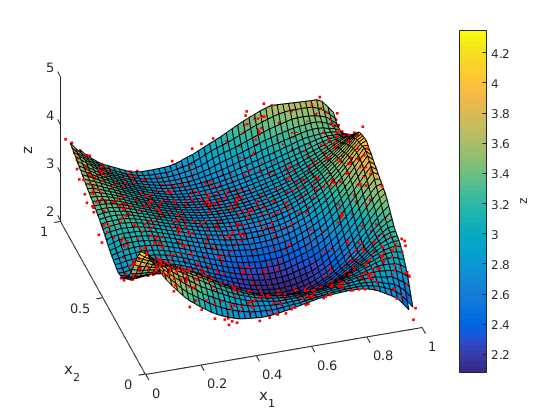
\includegraphics[height=5cm]{figs/train_surface.png}
\end{minipage}\quad
\begin{minipage}{0.4\textwidth}
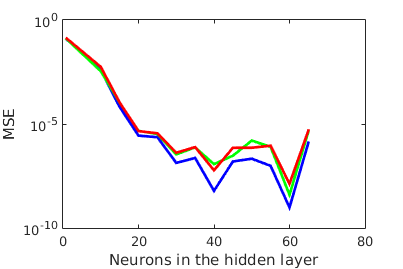
\includegraphics[height=5cm]{figs/performance_val.png}
\end{minipage}
\caption{Left: surface and data points in the training set. Right: Performance on the training, validation and test set as a function of the number of neurons in the hidden layer using $5000$ epochs. \label{fig:performance_val}}
\end{figure}

%\begin{figure}[tbh]
%\centering
%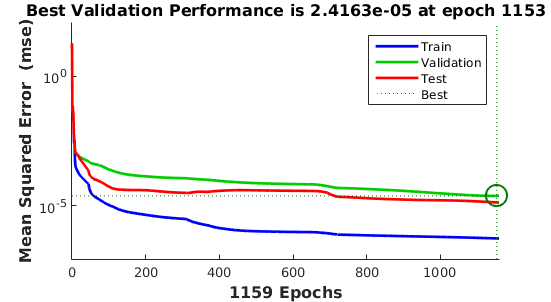
\includegraphics[height=5cm]{figs/MSE_final.png}
%\caption{Performance on the training, validation and test set as a function of the number of epochs in the training process. \label{fig:MSE_final}}
%\end{figure}

\begin{figure}[bth]
\centering
\begin{minipage}{0.5\textwidth}
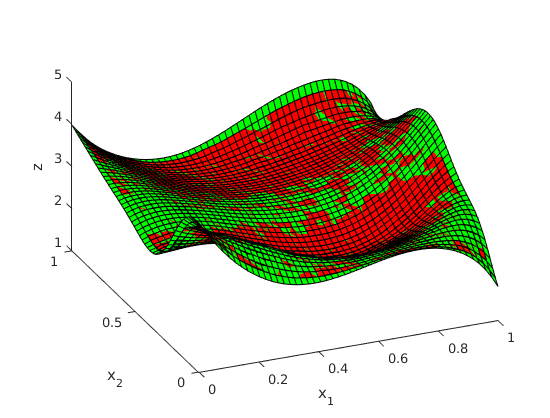
\includegraphics[height=5cm]{figs/NN_and_testsurf.png}
\end{minipage}%
\begin{minipage}{0.5\textwidth}
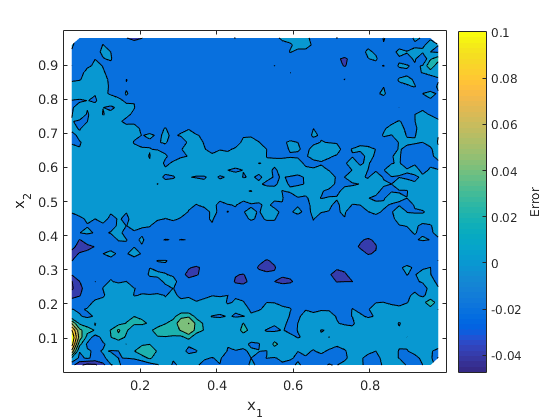
\includegraphics[height=5cm]{figs/NN_test_error.png}
\end{minipage}%
\caption{Left: Neural network (green) and test data (red) surface. The surfaces are almost indistinguishable. Right: Contour plot of the test set error. \label{fig:NN_and_testsurf}}
\end{figure}

The MSE on the test set of the resulting network is $2.2 \times 10^{-8}$. It clearly shows that the number of neurons is more than sufficient. We observe the pattern that the network has slightly higher values when the test-set interpolation is large, and smaller values when the interpolation function is small. Hence, more extremal values are obtained.
In the error surface plot in Fig.~\ref{fig:NN_and_testsurf}, the effect of a large number of neurons is clear: a small irregular oscillatory behaviour is observed.

To improve the results, we can use all of the provided data, instead of a subset of $3000$ data points. Since the number of training data entries is significantly larger, we also allow for $10$ additional neurons, resulting in $50$ neurons in the hidden layer. Also, the data division does not need to be equal for all sets. As a rule of thumb, one generally assumes 70:15:15 (or 60:20:20) for the train:validation:test set ratios. This changes the MSE test error to $1.46 \times 10^{-9}$.

Note that one could even improve these results by e.g.\ using cross validation, which allows one to use an even larger size training set. In $10$-fold cross validation for example, $90$ percent of the data can be used for training in each step. In the training-validation-test set strategy that we have applied above, $30$-$40$ percent of the data is used for checking generalization properties of the network.

Also, training multiple networks to approximate the function can in principle result in a better approximation. However, a certain bias was observed above. Since the current MSE is already low enough, we do not go into further details.

\section{PROJECT 2: Classification of wine data}\label{sec:classification}
According to my student number, I classify data sets $5$ and $6$. Since it is not given whether or not the wine data is linearly separable, we use a non-linear model. We now use a \texttt{tansig} transfer function in the output layer, since this restricts the output to the domain $[-1,1]$ and the target output is in the format of $\pm 1$. 
%We rescale the attributes to standardized values in order to make it independent of the scale of the data attributes. 
$15$ neurons in the hidden layer is optimal to classify the validation data. Using this architecture, a CCR of $0.737$  and $0.724$ is obtained for the validation and test set respectively. This might indicate that the two wine classes have a significant overlap in their attribute space. The effect of standardization of the data in this case appeared to have a rather negative effect.


\begin{figure}[htb]
\begin{minipage}{0.5\textwidth}
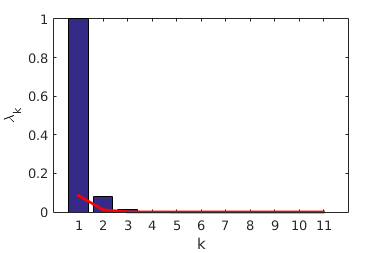
\includegraphics[height=4cm]{figs/eigenvalues_non-standardized.png}
\end{minipage}%
\begin{minipage}{0.5\textwidth}
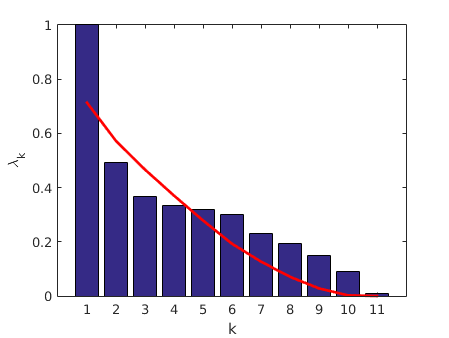
\includegraphics[height=4cm]{figs/eigenvalues.png}
\end{minipage}%
\caption{Eigenvalues of the $11\times11$ covariance matrix. The left and right panel show the result for the original and standardized data respectively. The red line indicates the cumulative sum of the remaining (k+1):end eigenvalues, which is proportional to the reconstruction error. \label{fig:eigenvalues}}
\end{figure}

Next, the data is projected onto its lower dimensional principle component basis and reconstructed afterwards. The eigenvalue spectrum of the covariance matrix is depicted in Fig.~\ref{fig:eigenvalues}. Prior to computing the covariance matrix, we rescale the data such that all attributes have zero mean and unit standard deviation. The effect of this rescaling results in a CCR difference of $3-6 \%$ in the final results (without standardization, we obtain $0.704$ and $68.4$ for the CCR of the validation and test set respectively). The scaled eigenvalue spectrum does not show a clear dominant principle component. We also show the non-standardized eigenvalue spectrum, which shows that only a single component dominates the spectrum. By rescaling the data, other features are emphasized. Note that the dominant eigenvalue might very well be related to the choice of attribute units. Hence, it makes sense to rescale the data before performing PCA.

There is no clear indication that the standardized data lives on a low-dimensional subspace. We take a reconstruction error of $10\%$, which corresponds to an $8$ dimensional basis. $11$ hidden neurons minimize the CCR of the validation set, which is less than before, as expected. Using this approach, a validation and test set CCR of $0.754$ and $0.717$ is obtained. Hence, there is a CCR increase of $5 \%$ for the validation set, while test set CCR is almost constant.
Hence, by linearly projecting the data onto a lower dimensional space, an insignificant classification improvement is realized. By rescaling the cata, the PCA analysis in principle corresponds to the original PCA, where the covariance matrix is substituted by the correlation matrix, which is dimensionless.

We remark that the possibility of overfitting is very real in this classification assignment. One can obtain an almost perfect CCR on the training set, while the test CCR is very low.

We have tested the effect of an additional hidden layer, since these are known to be beneficial in complex classification problems. The architectures $[10~10]$, $[15~15]$ and $[20~20]$ and even architectures with more than 2 hidden layers did not improve the results and resulted in at most the CCR ratios of the single-layer network. Hence, the additional non-linearity of the hidden layers does not improve the classification.

In principle, one of the reasons the PCA has a small effect can be due to the fact that it is organised in input space in such a way that linear PCA does not work. Hence, in principle other methods for PCA should be tested.

\newpage
\section{PROJECT 3: Character recognition}\label{sec:hopfield}
\subsection{Hopfield network}
\begin{figure}[htb]
\centering
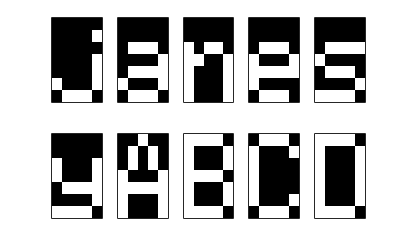
\includegraphics[width=10cm]{figs/letters.png}
\caption{First 10 of the 32 letters that are used in the character recognition exercise.\label{fig:letters}}
\end{figure}
In this section we train a Hopfield network to reconstruct the states in Fig.~\ref{fig:letters} from a distorted version of these characters. Hopfield networks are generated by providing them the undistorted images. 

\begin{figure}[htb]
\centering
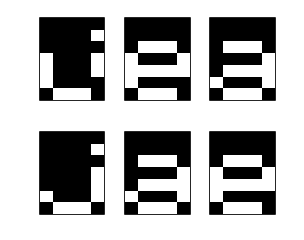
\includegraphics[width=8cm]{figs/wrong_states.png}
\caption{Incorrectly reconstructed characters (top row) with corresponding input (bottom row).\label{fig:wrong_states}}
\end{figure}

Figure~\ref{fig:wrong_states} illustrates a number of incorrectly reconstructed states with corresponding undistorted input. The `e' and `a' characters are often interchanged in the reconstruction. This is related to the fact that these characters have many pixels with the same value, and hence a similar shape. This means that the ridge in the energy function between these two attractor states is lower than the 3-pixel distortion. 
The incorrectly returned `j' character shows a spurious state which is a linear combination of multiple characters.
These cases are obtained when allowing for a sufficiently large number of time steps ($1000$). This allows one to observe the spurious states that are inherent to the system, rather than states that have not yet converged.

\begin{figure}[htb]
\centering
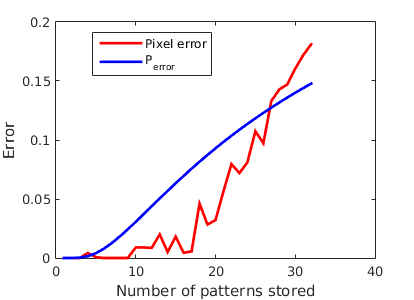
\includegraphics[width=8cm]{figs/Error_ifo_P.png}
\caption{Total pixel error (red),normalized over the number of states generated and total pixels in an image (35), and the theoretical prediction curve based on the Hebb rule (blue).\label{fig:error_ifo_P}}
\end{figure}

We now determine how the number of patterns stored influence the number of erroneously restored characters. For each case of $P$ stored patterns, we create a Hopfield network and generate a sufficient number of 3-pixel distorted images. These are then reconstructed, after which we calculate the number of pixels that do not correspond to the original image. The results are shown in Fig.~\ref{fig:error_ifo_P}. On can observe a steep rise in the reconstructed pixel error after $P=17$. Hence, $17$ stored patterns is the critical loading capacity of the network. Naturally, when the number of distorted pixels is increased, this number is expected to decrease. For $P$ larger than the critical loading capacity, the large number of spurious states and the small basins of attraction of attractor state do not allow for a reliable character restoration.

One can theoretically predict the dependence of the reconstruction error as a function of the number of patterns stored, using Hebbs' rule for uncorrelated patters. The prediction curve is also shown in Fig.~\ref{fig:error_ifo_P}. If we assume a large $P$ and large $N$, we obtain an estimated $P_{\textrm{error}}$
\begin{equation}
P_{\textrm{error}} = \frac{1}{\sqrt{2 \pi} \sigma} \int_{1}^{+\infty} e^{\frac{-x^2}{2 \sigma^2}} dx \,,
\end{equation}
where $\sigma=\sqrt{P/N}$. Hence, a first approximation is that $P$ and $N$ are large, which is not actually the case here. However, both the prediction and simulation show the same (expected) behaviour: first a flat $P$ dependence, followed by a steep rise. One can estimate the storage capacity from
\begin{equation}\label{eq:pmax}
P_{\max} = N/(4 \log N) =2.46 \,.
\end{equation}
Hence, for 2 or less stored patterns, the Hopfield should be able to perfectly reconstruct the distorted images. It can be shown\footnote{D.~J.~  Amit,  H.~Gutfreund,  and  H.~Sompolinsky.  Statistical  Mechanics  of  Neural  Networks  near Saturation. Annals.~of Physics 173, pp30-67, 1985} theoretically that the storage capacity is $P = 0.138 N=4.83$, for which if $P$ is larger, the system might get stuck in spurious local minima.

One way to resolve the issue of incorrectly reconstructed images, is to increase the number of pixels in each  image. In the case at hand, each image is determined by $35$ pixels. Hence, it was expected that the critical loading capacity would be relatively low. By increasing the number of pixels in an image, each character has more attributes by which it is characterized. This lowers the $P/N$ ratio. Using Eq.~\eqref{eq:pmax}, one can estimate the number of patterns that can be stored.

This is the obvious alternative to the current Hopfield network. In the next subsection we discuss another alternative which is more general and can easily be extended to more than $25$ characters. Since in principle, two-layered neural networks can reproduce any function, we can in principle form a perfect classifier (since we know \textit{all} 3 distorted images and hence can evaluate the underlying function everywhere) if and only if there are no overlapping distorted images. It requires, however, much more computing power compared to the Hopfield solution, since the Hopfield solution's training process is almost instantaneous. Note that many more solutions can be put forward, which all have their pros and cons. Naturally, also SVM's can be used in this case.

\subsection{Alternative solution to character recognition}
The Hopfield network for character recognition is ``only implemented in MATLAB for historical reasons''. Nowadays, many more, and better ANNs are available on the market. Not only can one choose the architecture of the network, but also the error determination can be chosen to optimize the problem. Another choice is which input is used to train the network. It has been shown that (as expected), a network performs better in character restoration if it is trained with distorted input images. This is clearly illustrated in an example by Matlab \footnote{\url{http://nl.mathworks.com/help/nnet/examples/character-recognition.html}}.

The opted network architecture is as follows: we generate a feedforward neural network with one hidden layer of $25$ neurons and an output layer of dimension equal to the number of patterns $P$ that are need to be stored. In the hidden layer, we use a \texttt{tansig} transfer function, while in the output layer, we use the \texttt{softmax} function. The final output is such that we put all output components to 0, except for the one with the maximum value, which is 1. Hence, we use one-hot encoding of the stored characters. This means that every character out of the $P$ stored characters is determined by a $P$-dimensional vector of zeros, except for a one in a unique place. Hence, also the actual characters must be stored such that one can return a character instead of this vector.  Note that the input still takes the $35$ pixels as in the original Hopfield network. In the syllabus a similar approach is discussed where the Hamming distance is used to select the final character when the image output vector results in an undetermined result. However, using the softmax function, we almost never find inconclusive results. 

One-hot encoding is feasible if the number of patterns stored is not too large, since the size of the output layer is equal to the size of the alphabet to be stored.

In the previous subsection we showed that the ``e'' and ``a'' are difficult for the Hopfield network to restore correctly, since these characters have very similar features. Hence, if one would create a network that uses an $N=35$ dimensional output, we know a priori that similar problems would be faced, since these characters are only separated by a small distance in output space. In one hot-encoding, the distance between two patterns in output space is $\sqrt{2}$, independent of whether they have similar patterns.

We train our network with $100$ distorted images of each letter to be stored. We vary the number of patterns and determine the number of incorrectly restored patterns as a function of the number of patterns stored. We use a constant $25$ hidden neurons for practical reasons. The results are shown in Fig.~\ref{fig:alternative_error}. A steady rise is observed as expected.
\begin{figure}
\centering
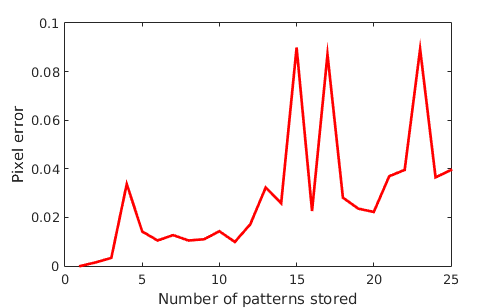
\includegraphics[width=8cm]{figs/alternative_error.png}
\caption{Percentage of false reconstructed images (not pixels as before) as a function of the number of patters stored.\label{fig:alternative_error}}
\end{figure}

Naturally, the network's performance can easily be improved by increasing the number of neurons and/or hidden layers. In addition, approximately $6500$ possible 3-pixel distortions of each letter. Hence, in theory all possibilities can be generated to form the training batch. However, substantial computing resources are required if batch-training is required. We will not go into further detail, since these calculations are hard to perform on a simple laptop.

\FloatBarrier
%%%%%%%%%%%%%%%%%%%%%%%%%%%%%%%%%%%%%%%%%%%%%%%%%%%%%%%%
\newpage
\appendix

%\lstset{style=Matlab-editor}
%
\lstset{language=Matlab,%
basicstyle=\small, %or \small or \footnotesize etc.
    %basicstyle=\color{red},
    breaklines=true,%
    morekeywords={matlab2tikz},
    keywordstyle=\color{blue},%
    morekeywords=[2]{1}, keywordstyle=[2]{\color{black}},
    identifierstyle=\color{black},%
    stringstyle=\color{mylilas},
    commentstyle=\color{mygreen},%
    showstringspaces=false,%without this there will be a symbol in the places where there is a space
    numbers=left,%
    numberstyle={\tiny \color{black}},% size of the numbers
    numbersep=9pt, % this defines how far the numbers are from the text
    emph=[1]{for,end,break},emphstyle=[1]\color{black}, %some words to emphasise
    %emph=[2]{word1,word2}, emphstyle=[2]{style},    
}

\section{Matlab code that implements the solutions}
\subsection{Regression (see Section \ref{sec:regression})}
\subsubsection{Main code}
\lstinputlisting{../project/regression/regression_project.m}
\subsection{Classification (see Section \ref{sec:classification})}
\subsubsection{Main code}
\lstinputlisting{../project/classification/classification.m}
\subsubsection{PCA related}
\lstinputlisting{../project/classification/doPCA.m}
\subsection{Character recognition (see Section \ref{sec:hopfield})}
\subsubsection{Main code}
\lstinputlisting{../project/hopfield/hopfield.m}
\subsubsection{Image distortion}
\lstinputlisting{../project/hopfield/DistortImage.m}
\subsubsection{Name generation}
\lstinputlisting{../project/hopfield/GenerateName.m}

\subsubsection{Alternative to Hopfield}
\lstinputlisting{../project/hopfield/alternative.m}




\end{document}